\newcommand{\da}{\Delta a}         % cell area or arclength in 2D
\newcommand{\das}{\overline{\da}}  % smoothed cell area
\newcommand{\xr}{{\bf xr}}
\newcommand{\xs}{{\bf xs}}
\newcommand{\xt}{{\bf xt}}
\newcommand{\xrr}{{\bf xrr}}
\newcommand{\xss}{{\bf xss}}

\newcommand{\ds}{{\bf ds}}
\newcommand{\dss}{{\bf dss}}



\section{HyperbolicMapping}

The HyperbolicMapping can be used to generate surface and volume grids by marching
along or from a given reference curve or surface.
 
% This Mapping is still under development and subject to possibly severe changes.

See the Mapping monster manual~\cite{MAPPINGS} for a information on many other Mappings
as well as a description of Mappings in general.

{
\newcommand{\figWidthd}{9cm}
\newcommand{\trimfig}[2]{\trimPlot{#1}{#2}{.0}{.0}{.0}{.0}}
\begin{figure}[hbt]
\begin{center}
\begin{tikzpicture}[scale=1]
  \useasboundingbox (0,.5) rectangle (9.,8.5);  % set the bounding box (so we have less surrounding white space)
%
  \draw ( 0.0,0.) node[anchor=south west,xshift=-4pt,yshift=+0pt] {\trimfig{\figures/hypeScreen}{\figWidthd}};
%
 % \draw (current bounding box.south west) rectangle (current bounding box.north east);
% grid:
% \draw[step=1cm,gray] (0,0) grid (9,8);
\end{tikzpicture}
\end{center}
\caption{Snapshot of the hyperbolic grid generator. A surface grid is grown on a CAD
  model for an automobile. A starting curve is chosen and the grid is grown in both directions
   over the surface.} \label{fig:screenAsmo}
\end{figure}
}


\subsection{Hyperbolic Marching Equations}

\newcommand{\nvhat}{\hat{\nv}}


Let $(r,s,t)$ denote the parameter space (computational) coordinates.
Instead of taking parameter space to be the unit cube we instead take
the grid spacing in parameter space to be 1, $\Delta r = \Delta s =
\Delta t =1$. 

Given a surface $\xv_0(r,s)=\xv(r,s,t=0)$ we wish to generate a volume
grid, $\xv(r,s,t)$, so that the grid lines in the $t$-direction are
nearly orthogonal to the grid lines in the two other directions.  We
call $\xv(r,s,t=0)$ the initial front and think of the variable $t$ as
a time like variable.  If we have generated the grid to ``time''
$t=t_0$ we call $\xv(r,s,t_0)$ the current front.


The basic marching equations to determine $\xv(r,s,t)$ given $\xv(r,s,0)$ are defined by
the hyperbolic PDE
\begin{alignat*}{3}
   \xv_t &= S(r,s,t)~ \nv(r,s,t) \\
   \xv(r,s,0) &= \xv_0(r,s) &&\qquad \mbox{initial conditions} \\
   B(\xv(r,s,t))&=0 && \qquad \mbox{boundary conditions}
\end{alignat*}
where
\begin{alignat*}{3}
  \nv(r,s,t) &= {\xv_r \times \xv_s \over \| \xv_r \times \xv_s \|} &&\qquad\mbox{normal to the front} \\
  S(r,s,t) & &&\qquad\mbox{scalar speed function}  
\end{alignat*}
and the norm $\| \cdot \|$ is defined by
\[
  \| \fv \|^2  \equiv \fv \cdot \fv.
\]
These equations march the grid in the direction locally orthogonal to the current front. 
The speed function $S(r,s,t)$ determines how fast the front propagates; it can depend
on local properties of the front. 
Smoothing is also added to the equations so we actually solve a parabolic equation of the form
\[
    \xv_t = S(r,s,t) \nv  + \epsilon(r,s,t) ( \xv_{rr} + \xv_{ss} )
\]
To ensure that the front always propgates in the forward direction we require
$\nv\cdot\xv_t > 0$ or equivalently
\[
   \nv\cdot\Big( S(r,s,t) \nv  + \epsilon( \xv_{rr} + \xv_{ss}) \Big) > 0 
\]
In addition to smoothing the grid in the $(r,s)$ directions, the the
parabolic smoothing term will tend to slow the front where the
curvature is negative (i.e. $\nv\cdot(\xv_{rr}+\xv_{ss}) < 0$) and speed up the front where the curvature is
positive. Note that choosing too large a value for $\epsilon$ could cause the
front to propogate in the wrong direction resulting in negative
cell-volumes.  The speed function $S(r,s,t)$ and dissipation
coefficient $\epsilon$ should be specified so that we get a ``nice
grid''. A nice grid should not have any grid lines that cross, it should be reasonably orthogonal
and reasonably smooth. 


The marching equations can be solved with an implicit time marching algorithm.
To do this we first linearize the equations about the current front, $\xv(r,s,t^n)$, to obtain
an equation of the form
\[
  \xv_t = A(r,s,t)  \xv_r + B(r,s,t) \xv_s  + \epsilon( \xv_{rr} + \xv_{ss} ) + \fv(r,s,t)
\]
This equation can be solved using a $\theta-$scheme for $\xv(r,s,t^n)\approx \xv^n$,
\begin{align*}
  { \xv^{n+1} - \xv^n \over \Delta t} &= 
       \theta\left[ A(r,s,t^{n+1}) \xv_r^{n+1} + B(r,s,t^{n+1}) \xv_s^{n+1} 
           + \epsilon ( \xv_{rr}^{n+1} + \xv_{ss}^{n+1} )\right]  \\
 & + (1-\theta) \left[ A(r,s,t^{n}) \xv_r^{n} + B(r,s,t^{n}) \xv_s^{n} 
            + \epsilon ( \xv_{rr}^{n} + \xv_{ss}^{n} )\right] + \fv^n \\
  \fv^n &=  S^n \nv \mbox{??}
\end{align*}
where $\theta=1$ corresponds to backward-Euler. For efficiency we use
an approximate factorization to reduce the implicit matrix solve to a sequence
of block-tridiagonal solves. 

We now consider choices for the speed function, $S(r,s,t)$.
Following the approach of Steger-Chan we define the speed function based on the 
local cell-areas of the front,
\begin{align*}
 S_A(r,s,t) & =  d_0(t) ~\Delta t ~ \das / \da  \\
 d_0(t) \Delta t  &= \mbox{distance to march in a time step $\Delta t$, (approximate average value)} \\
 \da(r,s) &= \| \xv_r \times \xv_s \|  \qquad \mbox{proportional to the local area of the front}\\
 \das(r,s) &= \mbox{Locally averaged value of $\da(r,s)$}
\end{align*}
The speed function is proportional to the local cell area divided by a
locally average cell area.  The averaged cell area, $\das(r,s)$, is
computed by smoothing the cell area $\da(r,s)$ using a simple Jacobi
type interation.  As a result of using this speed function the grid
will tend to grow faster where the area of cells on the front are
smaller and slower where the grid cells are larger compared to the
local average. Asymptotically a front will tend toward a curve where
the surface areas are equal. For example, a front may tend to a sphere
or a plane in 3D, depending on the boundary conditions for the front.
Steger and Chan also use a sophisticated dissipation term as described in section~\ref{sec:StegerChan}.

Following the approach of Sethian we could also choose the speed function proportional 
the the local curvature,
\begin{align*}
    S_c(r,s,t) &= (1-\epsilon_c \kappa(r,s,t)) \\
    \kappa(r,s,t) &= \mbox{local curvature}
\end{align*}
If $\epsilon_c>0$ then we are guaranteed that grid lines will not locally cross, although the front
could propogate in the wrong direction id $S_c$ becomes negative.
Here the curvature $\kappa$ causes the grid to move faster where the curvature is negative
and slower where it is positive. The hyperbolic grid generator allows one to use a combination
of the area based speed function and the curvature based spped function. 
The comnbined speed function is taken as the product of $S_A$ and $S_c$,
\begin{align*}
 S(r,s,t) & =  d_0(t) ~\Delta t ~ \das / \da ~~(1-\epsilon_c \kappa(r,s,t))
\end{align*}


% \[
%     \xv_t = {\nvhat \over \| \nvhat \|^2} ~ V(r,s,t)
% \]
% where $\nvhat$ is a vector that is locally normal to the front,
% \[
%     \nvhat = \xv_r \times \xv_s
% \]
% and where $V(r,s,t)$ is a specfied cell-volume distribution.
% For example we typically use
% \begin{align*}
%  V(r,s,t) & =  D \| \nvhat \| ~ \das / \da^{-1}  \\
%  \da(r,s) &= \| \xv_r \times \xv_s \|  \\
%  \das(r,s) &= \mbox{Locally averaged value of $\da(r,s)$}
% \end{align*}
% 
% 
% These equations will generate a grid where the grid lines in the $t$-direction will be
% orthogonal to the grid lines in the other two directions.
% 
% Smoothing is also added to the equations so we actually solve something like
% \[
%     \xv_t = {\nvhat \over \| \nvhat \|^2} ~ V(r,s,t) + \epsilon( \xv_{rr} + \xv_{ss} )
% \]

For 2D volume grids or 3D surface grids 
there is also an option to blend the solution obtained from the above equation with
a distribution of points based on equidistributing a weight function based on the
arclength and curvature. If we equidistrubte the arclength, for example, we will obtain
a distribution of points, $\xv^E$, that are equally spaced in arclength. A new front is defined
by averaging the equidistributed points with the points determined by using the speed function.
\[
  \tilde{\xv}(r,s,t) = (1-\omega^E) \xv(r,s,t) + \omega^E \xv^E(\xv(r,s,t)) 
\]
The equidistributed points are determined by a weight function 
\begin{align*}
    w(r) &= \alpha^A \| \xv_r \| / \| \xv_r \|_\infty + \alpha^C \| \xv_{rr} \| / \| \xv_{rr} \|_\infty \\
\end{align*}
where $\| \fv \|_\infty = \max_r \| \fv(r) \|$.
The weight function is equidsitributed over the unit interval to determine 
positions $r^E_i \in [0,1]$, $i=1,2,\ldots,N$, $r^E_{i+1} > r^E_i$, such that
\[
    \int_{r^E_i}^{r^E_{i+1}} w dr = {1\over N} \int_0^1 w dr
\]
This last equation expresses the condition that the weight function is equidistributed.
The new grid points positions are computed by evaluating the curve, $\cv(r)$, defining the
current front at the new parameter positions $r^E_i$,
\[
    \xv^E := \cv( \rv^E ) \cc{re-evaluate the curve at the new positions}
\]


Following Steger, the hyperbolic marching equations can be cast in an alternative form 
\begin{align}
   \xv_r \cdot \xv_t & = 0 \\
   \xv_s \cdot \xv_t & = 0 \\
   \xv_r \times \xv_s \cdot \xv_t & = \Delta V(r,s,t)  
\end{align}   
The first two equations specify the orthogonality conditions while the 
last equation specifies the local volume of the cell, $\Delta V$.
We can solve these equations for $\xv_t$ and we see that the solution is defined by locally
marching along rays that move in the normal direction:
\begin{align*}
  \xv_t(r,s,t) & = {\xv_r(r,s,t) \times \xv_s(r,s,t) \over \| \xv_r(r,s,t) \times \xv_s(r,s,t) \|^2} \Delta V \\
               & = {\Delta V  \over \| \xv_r(r,s,t) \times \xv_s(r,s,t) \| } ~~ \nv(r,s,t)\\
   \nv(r,s,t) & = {\xv_r(r,s,t) \times \xv_s(r,s,t) \over \| \xv_r(r,s,t) \times \xv_s(r,s,t) \|} \label{hype2}
\end{align*} 
and thus we can identify the speed function
\[
    S(r,s,t) = {\Delta V  \over \| \xv_r(r,s,t) \times \xv_s(r,s,t) \| }
\]
If we choose $\Delta V(r,s,t)= c \| \xv_r(r,s,t) \times \xv_s(r,s,t) \|$, for a constant $c$,
then the grid lines in the marching direction will just be straight lines parallel to the 
normal of the original surface.
Of course the grid generated by this system may develop singularities, if any part
of the original surface is concave. To avoid this problem extra smoothing is added.

If we choose $\Delta V(r,s,t)= c$ then the grid spacing in the normal direction will
be inversely proportional to the local surface cell area. Thus the grid will grow
fastest where the cells are small.


The basic marching distance depends on the type of stretching, the total distance to march $D$, and the
number of steps to march, $N$:
\begin{align*}
   \dv_\iv^n  &= { D \over N}  \qquad\mbox{constant spacing} \\
   \dv_\iv^n  &= D~ \alpha^n {\alpha -1 \over \alpha^{N+1} -1} \qquad\mbox{geometric stretching}
\end{align*}
The volume element appearing in the marching step is a product of the marching distance
times the ratio of the averaged area element $\das_\iv$ to the area element $\da_\iv$
\[
\Delta V_\iv = \dv_\iv^n { \da_\iv \over \das_\iv} \qquad\mbox{: volume element}
\]

% The normal at each vertex is computed as an average of the cell centred normals  of the neighbouring cells.
% The area element is also defined in a similar way.
% \begin{alignat*}{2}
% \hat{\nv}_{\iv+\half} &= (\xv_{i+1}-\xv_i)\times (\xv_{j+1}-\xv_j)  &\qquad& \mbox{cell centred normal (unnormalized)} \\
% \nv_{\iv+\half} &= \hat{\nv}_{\iv+\half} / \| \hat{\nv}_{\iv+\half} \|  &\qquad& \mbox{cell centred normal} \\
% \hat{\nv}_{ij} &= {1\over4}( \nv_{i-\half,j-\half}+\nv_{i+\half,j-\half}+
%                              \nv_{i-\half,j+\half}+\nv_{i+\half,j+\half} ) \\
% \nv_{ij} &= \hat{\nv}_{ij}/\| \hat{\nv}_{ij} \|   &\qquad& \mbox{vertex centred normal} \\
% \Delta a_{\iv+\half} &= \| \hat{\nv}_{\iv+\half} \|    &\qquad& \mbox{cell centred  area element} \\
% \Delta a_{ij} &= {1\over4}( a_{i-\half,j-\half}+a_{i+\half,j-\half}+
%                              a_{i-\half,j+\half}+a_{i+\half,j+\half} ) &\qquad& \mbox{vertex centred area element} \\
% \Delta \hat{a}_{ij} &= \Sv^\nu a_{ij}  &\qquad& \mbox{smoothed area elements} \\
% \end{alignat*}


Parameters appearing in the code are
\begin{description}
  \item[number of volume smooths] : number of times we smooth $\da_\iv$ to obtain $\das_\iv$.
  \item[uniform dissipation coefficient] : $\epsilon$, coefficient of the parabolic terms.
  \item[implicit coefficient] : $\theta$ coefficient of implicit time stepping.
  \item[equidistribution] : weight factor for the equidistributed approach.
  \item[arclength weight] : $\alpha_A$ weight for arclength in equidistribution weight function
  \item[curvature weight] : $\alpha_C$ weight for curvature in equidistribution weight function
  \item[curvature speed] : $\epsilon_c$ weight factor for the curvature dependent speed function.
\end{description}

\clearpage
\subsection{Algorithm}\index{algorithm}

Here is a summary of the algorithm 

\begin{flushleft}
\bc{Notation:}\\
 $n_d$ \cc{domain dimension, $n_d\equiv2$ for 2D volume grids or 3D surface grids, $n_d\equiv3$ for 3D volume grids}\\
  $\Cv$ \cc{starting surface (or starting curve) }\\
  $\Rv$ \cc{reference surface for surface grid generation}\\
  $\da_\iv$ \cc{local surface area (arclength in 2D)}\\
  $\das_\iv$ \cc{smoothed surface area (smoothed arclength in 2D)}\\
  $\nv_\iv$ \cc{normal}\\
  $D$ \cc{marching distance}\\
  $N$ \cc{number of steps to march}\\
  $\iv$ \cc{multi-index $\iv=(i_1,i_2)$ for 3D volume grids,  or $\iv=(i_1)$ for 2D grids or 3D surface grids.}
\end{flushleft}


% \begin{tabbing}
% 1234567890 \= 1234 \= 1234 \= 123456789012345678901234567890 \= 1234  \= 1234 \= 1234 \=  \kill  % define tabs
% \> $\xv^0=\Cv(\rv)$ \>\>\>: evaluate the initial curve                 \\
% \> {\bf if} surfaceGrid           \\
% \>\> $\xv^0 = \Pv(\xv^0)$ \>\>: project onto the reference surface        \\
% \> {\bf for} n=0,1,...,N     \\
% \>\>  $\nv=(\xv_r\times\xv_s)/\|\xv_r\times\xv_s\|$              \>\>: compute the normal \\
% \>\>  $\Delta a=\Sv^{\nu} \| \xv_r\times\xv_s \|$              \>\>: compute and smooth the surface areas   \\
% \>\>  $\Delta s^n = \Lv(\Delta a,n)$                            \>\> : compute step length \\
% \>\>  $\Delta s=\Delta s (1-\epsilon\kappa)$                  \>\> : adjust step length by curvature\\
% \>\> $M_1 = I + C_0^{-1}A_0 \delta_r - \epsilon_i \Delta_r $  \>\>: form implicit time stepping matrices \\
% \>\> $\rv = \Delta V(\Delta s, \Delta a) \nv + \epsilon \Delta_\rv \xv$ \>\> : rhs \\
% \>\> $\Delta\xv \leftarrow  M_2^{-1}M_1^{-1}\rv$                               \>\>: solve for correction \\
% \>\> $\xv^{n+1} = \xv^n + \Delta \xv$ \\
% \>\> apply boundary conditions \\
% \>\> {\bf if} surfaceGrid           \\
% \>\>\> $\xv^{n+1} = \Pv(\xv^{n+1})$ \>: project onto the reference surface        \\
% \> {\bf end for}
% \end{tabbing}



\begin{algorithm}
\caption{Hyperbolic grid generator: Generate a volume grid in 2D or 3D or a surface grid in 3D}
\begin{algorithmic}[1]
\Function{{\bf generate}}{~}
  \State $\xv^0_\iv := \Cv(\rv_\iv)$ \Comment{evaluate the starting surface (starting curve if $n_d\equiv2$)}
  \If{ this is a surface-grid}
    \State \bc{projectInitialCurveOntoReferenceSurface}($\xv^0, \nv_\iv, \xt; \Rv$)
  \EndIf
  \State
  \State hyperbolic marching steps:
  \For{$n=0,1,...,N$}

    \State \bc{getNormalAndSurfaceArea}($\xv^n, \nv, \da, \das, \xr, \xs$)
    \State \bc{getDistanceToStep}($\dv_\iv$)  \cc{get marching distance}
    \State \bc{getCurvatureDependentSpeed}($\dv_\iv$)  \cc{adjust marching distance for curvature}

    \If{$n\equiv 0$ and this is not a surface grid}
      \State $\xt_\iv := \dv_\iv~({\das_\iv / \da_\iv})~\nv_\iv$ \Comment{linearize about this value of $\xv_t$}
    \EndIf

    \State Form the right-hand-side:
    \State $\rv_\iv := \dv_\iv~({\das_\iv / \da_\iv})~\nv_\iv + \epsilon_e \Delta_{+r}\Delta_{-r} \xv^n_\iv + \epsilon_e \Delta_{+s}\Delta_{-s} \xv^n_\iv$

    \State $A := A(\xr,\xs,\xt)$ \Comment{linearized coefficient matrix for implicit time stepping}
    \State $B := B(\xr,\xs,\xt)$
    \Comment{form implicit time stepping matrices:}

    \State $M_1 = I + A \Delta_{0r} - \epsilon_i \Delta_{+r}\Delta_{-r}$
    \State $ M_2 = I + B \Delta_{0s} - \epsilon_i \Delta_{+s}\Delta_{-s}$ \Comment{$M_2=I$ for $n_d\equiv2$}

    \State $\vv :=  M_2^{-1}M_1^{-1} \rv$ \Comment{solve for the correction}

    \State $\xv^{n+1}_\iv := \xv^n_\iv + \vv_\iv$

    \State 
    \State Next apply BC's and optionally adjust for equidistribution.
    \State For surface grids project $\xv^{n+1}$ onto the reference surface:
    \State \bc{applyBoundaryConditions}($\xv^{n+1}$)  
  
    \State 
    \State $\xt_\iv := \xv^{n+1}_\iv - \xv^n_\iv$  \Comment{linearize about this value of $\xv_t$}

  \EndFor
\EndFunction
\end{algorithmic}
\end{algorithm}




\begin{algorithm}
\caption{Project the initial curve onto the reference surface and determine the initial normal}
\begin{algorithmic}[1]
 \Function{{\bf projectInitialCurveOntoReferenceSurface}}{$\xv^0, \nv_\iv, \xt; \Rv$}
    \State Project initial curve onto the reference surface, compute normal
    \State \bc{project}($\xv^0, \nv_\iv; \Rv$)

    \State In case the initial curve lies on a {\em edge} in the reference surface where
    \State the normal is ill-defined, take a small initial step and then recompute the normal.
    \State \bc{getNormalAndSurfaceArea}($\xv^0, \nv, \da, \das$)

    \State \bc{getDistanceToStep}($\dv_\iv$)  \Comment{get marching distance}

    \State  $\delta = .1$  \cc{take this fraction of a step}
    \State $\xv^1_\iv := \xv^0_\iv + \delta~\dv_\iv~({\das_\iv / \das_\iv})~\nv^0_\iv$   \Comment{take a small step}

    \State \bc{applyBoundaryConditions}($\xv^1, \nv$)  \Comment{this will also project onto the reference surface}

    \State $\xt_\iv := (\xv^1_\iv-\xv^0_\iv)/\delta$  \Comment{linearize about this value of $\xv_t$}
\EndFunction
\end{algorithmic}
\end{algorithm}



\begin{algorithm}
\caption{Determine the normal and surface area}
\begin{algorithmic}[1]
 \Function{{\bf getNormalAndSurfaceArea}}{$\xv^n, \nv,  \da, \das, \xr, \xs$}
  \State Param: $\xv^n$ \cc{position of the front}
  \State Param: $\da_\iv$ \cc{(output) vertex centred area element}
  \State Param: $\das_\iv$ \cc{(output) vertex centred averaged area element}
  \State Param: $\xr$ \cc{(output) }
  \State Param: $\xs$ \cc{(input/output) : for a surface grid $\xs$ defined on input as the normal to the surface.}
  \State 
  \State $\hat{\nv}_{\iv+\half} := (\xv_{i+1}-\xv_i)\times (\xv_{j+1}-\xv_j)$  \Comment{unnormalized face centred normal}

  \State $\nv_{\iv+\half} := \hat{\nv}_{\iv+\half} / \| \hat{\nv}_{\iv+\half} \|$  \Comment{face centred normal} 

  \State $\hat{\nv}_\iv := {1\over4}( \nv_{i_1-\half,i_2-\half}+\nv_{i_1+\half,i_2-\half}+\nv_{i_1-\half,i_2+\half}+\nv_{i_1+\half,i_2+\half} ) $

  \State $\nv_\iv := \hat{\nv}_\iv/\| \hat{\nv}_\iv \|$   \Comment{vertex centred normal}

  \State $\Delta a_{\iv+\half} := \| \hat{\nv}_{\iv+\half} \|$    \Comment{cell centred  area element} 
  \State \mbox{vertex centred area element:}
  \State $\Delta a_{ij} := {1\over4}( \Delta a_{i-\half,i_2-\half}+\Delta a_{i+\half,i_2-\half}+\Delta a_{i-\half,i_2+\half}+\Delta a_{i+\half,i_2+\half} )$

  \State 
  \State \bc{apply special boundary conditions to normals}
  \If{trailing edge boundary condition}
     \State \mbox{set normal to the trailing edge direction}
  \ElsIf{boundary matches to an adjacent surface}
     \State \mbox{project the normal at the boundary to be tangent to the boundary condition surface}
     \State \mbox{$\nv^B_\iv$ : normal to the boundary condition surface}
     \State $\nv_\iv := \nv_\iv - (\nv_\iv \cdot \nv^B_\iv ) \nv^B_\iv$ \Comment{for boundary points}
     \State $\nv_\iv := \nv_\iv / \| \nv_\iv \|$
  \ElsIf{boundaryCondition=fixXfloatYZ or boundaryCondition=fixYfloatXZ etc.}
     \State \mbox{adjust normal to be consistent with the boundary condition}
  \EndIf

  \State
  \State \bc{blend nearby normals with the boundary normal}
  \For{$m=1,2,\ldots,\mbox{numberOfLinesToBlend}$}
    \State $\omega = m/(\mbox{numberOfLinesToBlend}+1)$
    \State $\nv_{\iv+m} = \omega \nv_{\iv+m} + (1-\omega) \nv_\iv$
    \State $\nv_{\iv+m} = \nv_{\iv+m} / \| \nv_{\iv+m} \|$
  \EndFor

  \State
  \State \mbox{Compute smoothed area elements:} 
  \State $\omega := .1625$ \Comment{under-relaxation parameter}
  \State $\das_\iv := \da_\iv$
  \For{$m=1,2,\ldots,\mbox{numberOfVolumeSmoothingIterations}$}
    \State $das_\iv := (1-\omega) \das_\iv + \omega/4 ( \das_{i_1+1} + \das_{i_1-1} + \das_{i_2+1} + \das_{i_2-1} )$
  \EndFor

  \State $\xr_\iv := \half ( \xv_{i_1+1}-\xv_{i_1-1})$

  \If{$n_d\equiv 2$}
    \State $\xs_\iv := \half ( \xv_{i_2+1}-\xv_{i_2-1})$
  \EndIf
\EndFunction
\end{algorithmic}
\end{algorithm}


\newcommand{\ig}{{\bf ig}}
\newcommand{\ib}{{\bf ib}}

\begin{algorithm}
\caption{Apply boundary conditions.}
\begin{algorithmic}[1]
 \Function{{\bf applyBoundaryConditions}}{$\xv^n, \nv$}
  \State \bc{Purpose} \cc{Apply boundary conditions to the current front. Optionally equidsitribute lines.}
  \State   \mbox{For surface grids, project the front onto the reference surface}
  \State Param: \ig \cc{Denotes the index for ghost points}
  \State Param: \ib \cc{Denotes the index for boundary points}
  \State 
  \If{boundaryCondition == freeFloating}
    \State  $\xv_\ig = 2 \xv_\ib - \xv_{\ib+1}$ \Comment{extrapolate ghost line}
  \ElsIf{boundaryCondition == outwardSplay}

  \ElsIf{boundaryCondition == fixXfloatYZ}

  \ElsIf{boundaryCondition == periodic }

  \ElsIf{boundaryCondition == matchToMapping}

    \State Project the boundary points onto the boundary mapping

   \State  $\Bv := \mbox{mapping defining the boundary that we should match to}$
   \State  $\Bv.\bc{project}(\xv_\ib)$

  \EndIf

  \State 
  \State \bc{equidistributeGridLines}( $\xv^{n+1}$ )

  \State 
  \If{this is a surface-grid}
    \State \bc{project}($\xv^0, \nv_\iv; \Rv$)
  \EndIf
  \State 
  \State \bc{apply periodic boundary conditions}

\EndFunction
\end{algorithmic}
\end{algorithm}


\begin{algorithm}
\caption{Get the distance to step.}
\begin{algorithmic}[1]
 \Function{{\bf getDistanceToStep}}{$\dv$}
  \State \bc{Purpose} \cc{Return the current suggested distance to step}
  \State Param: n \cc{current step number}
  \State Param: N \cc{number of lines to march}
  \State Param: D \cc{distance to march}
  \State Param: $\alpha$ \cc{geometric stretching factor}
  \State 
  \If{constant spacing}
   \State $\dv = D/N$
  \ElsIf{geometric spacing}
    \State $\dv = D \alpha^n { \alpha -1 \over \alpha^{N+1} -1 }$
  \EndIf

\EndFunction
\end{algorithmic}
\end{algorithm}



\begin{algorithm}
\caption{Equidistribute the grid lines.}
\begin{algorithmic}[1]
\Function{{\bf equidistributeGridLines}}{$\xv^n$}
  \State \bc{Purpose} \cc{Adjust points based on the arclength and curvature}
  \State Param: $\xv^n$ \cc{current grid point positions}
  \State Param: $\cv$ \cc{A curve that interpolates the points $\xv^n$}
  \State Param: $\omega^E$ \cc{equidistribution weight, $0\le \omega^E \le 1$}
  \State Param: $\alpha^A$ \cc{equidistribution arclength weight}
  \State Param: $\alpha^C$ \cc{equidistribution curvature weight}
  \State 
  \If{$n_d \equiv 2$ \cc{only used for domain dimension equal to 2}}

    \State \cc{compute a weight function based on arclength and curvature}

    \State $\ds_{i_1+\half} := \| \xv_{i_1+1} - \xv_{i_1} \|$  \Comment{chord length}
    \State $\dss_{i_1} :=\| \xv_{i_1+1} - 2\xv_{i_1} + \xv_{i_1-1}\|$
  
    \State $w_{i_1+\half} := \alpha^A \ds_{i_1+\half} / \| \ds \|_\infty + \alpha^C \dss_{i_1+\half} / \| \dss \|_\infty$

    \State \mbox{equidistribute the weight function: determine positions $\rv^E_i \in [0,1]$ such that:}

    \State $\int_{\rv^E_i}^{\rv^E_{i+1}} w dr = {1\over N} \int_0^1 w dr$

    \State $\xv^E := \cv( \rv^E )$ \Comment{re-evaluate the curve at the new positions}

    \State \cc{weighted average of current positions and equidistributed positions}
    \State $\xv^n := (1-\omega^E) \xv^n + \omega^E \xv^E$

  \EndIf

\EndFunction
\end{algorithmic}
\end{algorithm}


\clearpage
% --------------------------------------------------------------------------------------------------------------------
\section{Steger-Chan Hyperbolic Marching}\label{sec:StegerChan}

The approach discussed here follows {\sl Enhancements of a Three-Dimensional Hyperbolic Grid
Generation Scheme} by Chan and Steger\cite{Chan92} and
{\sl A Hyperbolic Surface Grid Generation Scheme and Its Applications} by Chan and Buning\cite{Chan94}.


Notation: Unit square coodinates $(r,s,t)$ with marching direction along $t$. 

Given a surface $\xv(r,s,t=0)$ we wish to generate a volume grid, $\xv(r,s,t)$, that extends
in a direction that is nearly normal to the surface. To do this we choose $\xv_t$ to satisfy
\begin{align}
   \xv_r \cdot \xv_t & = 0 \\
   \xv_s \cdot \xv_t & = 0 \\
   \xv_r \times \xv_s \cdot \xv_t & = \Delta V(r,s,t)  \label{hype1}
\end{align}   
where we have added the additional condition specifying the local volume of the cell.

To avoid a small time step in advancing the front we linearize and use an implicit time stepping method.
We can linearize about the state $\xv^0$ (which we will later take to be the current time step).
It is easier if we linearize the equations in their original form of equation~\ref{hype1},
\begin{align*}
    \xv_t^0 \cdot \xv_r + \xv_r^0 \cdot \xv_t & = 0 \\
   \xv_t^0 \cdot \xv_s + \xv_s^0 \cdot \xv_t & = 0 \\
  (\xv_s^0 \times \xv_t^0) \cdot \xv_r + (\xv_t^0 \times \xv_r^0) \cdot \xv_s +
         (\xv_r^0 \times \xv_s^0) \cdot \xv_t & = \Delta V(r,s,t) + 2\Delta V^0
\end{align*}  
or in matrix form
\[
   A_0 \xv_r + B_0 \xv_s + C_0 \xv_t = \fv 
\]
or
\[
\begin{bmatrix} (\xv_t^0)^T \\ 0 \\ (\xv_s^0 \times \xv_t^0)^T \end{bmatrix} \xv_r +
\begin{bmatrix} 0 \\  (\xv_t^0)^T \\ (\xv_t^0 \times \xv_r^0)^T \end{bmatrix} \xv_s +
\begin{bmatrix} (\xv_r^0)^T \\ (\xv_s^0)^T \\ (\xv_r^0 \times \xv_s^0)^T \end{bmatrix} \xv_t
= \begin{bmatrix} 0 \\ 0 \\ V(r,s,t) + 2\Delta V^0 \end{bmatrix}
\]
or
\[
   \xv_t= - C_0^{-1}A_0 \xv_r - C_0^{-1}B_0 \xv_s +  C_0^{-1}\fv
\]
Writing this in incremental form
\[
   A_0 (\xv_r-\xv_r^0) + B_0 (\xv_s-\xv_s^0) + C_0 \xv_t = \gv = \begin{bmatrix} 0 \\ 0 \\ V(r,s,t) \end{bmatrix}
\]
\newcommand{\dxv}{\delta\xv}
If $\dxv = \xv^{n+1} - \xv^n$ then using the approximation $\xv_t\approx\xv^{n+1} - \xv^n$ ($\Delta t=1$)
\[
   \dxv= - C_0^{-1}A_0 ~\dxv_r - C_0^{-1}B_0 ~\dxv_s +  C_0^{-1}\gv
\]
Discretizing with backward Euler
\[
   [ I + C_0^{-1}A_0 \Delta_{0r} + C_0^{-1}B_0 \Delta_{0s} ] ~\dxv = C_0^{-1}\gv
\]
approximate factorization
\[
   [ I + C_0^{-1}A_0 \Delta_{0r}][I + C_0^{-1}B_0 \Delta_{0s} ] ~\dxv = C_0^{-1}\gv 
\]
Smoothing is added to this equation
\begin{align*}
   [ I + C_0^{-1}A_0 \Delta_{0r} - \epsilon_i \Delta_{+r}\Delta_{-r} ]
   [ I + C_0^{-1}B_0 \Delta_{0s} - \epsilon_i \Delta_{+s}\Delta_{-s} ] ~\dxv & = C_0^{-1}\gv  \\
        &+ \epsilon_e \Delta_{+r}\Delta_{-r} \xv^n + \epsilon_e \Delta_{+s}\Delta_{-s} \xv^n \\
        &+ D_r \xv^n + D_s \xv^n
\end{align*}
Note that the smoothing terms have components in the normal and tangential directions. The smoothing will
increase the step size in concave regions $\nv\cdot( \xv_{rr} + \xv_{ss} ) >0 $ and decrease the step size
in convex regions.

The cell volume can be computed to be the local area of the element times a user specified
step length,
\[
    \Delta V = \Delta L(r,s,t) \Delta A(r,s,t)
\]
where the step length may be chosen to stretch the grids lines in any desired way.
The area $\Delta A(r,s,t)$ is usually smoothed using a few Jacobi iterations.

The variable dissipation coefficients are defined by
\begin{align*}
  D_r  &= \epsilon_{er}(r,s,t) \Delta_{+r}\Delta_{-r} \\
 \epsilon_{er}(r,s,t) &= \epsilon_e R_r N_r \\
 N_r &= \| \xv_t \| / \| \xv_r \| \\
 R_r &= K^n {\overline d}^r_\iv a^r_\iv \\
\end{align*}
Scaling function, $K^n$,
\[
   K^n =  \begin{cases}
              \sqrt{ (n-1)/(n_{\rm{max}}-1) } & \text{if $2\le n \le n_{\rm{trans}}$} \\
              \sqrt{ (n_{\rm{trans}}-1)/(n_{\rm{max}}-1) } & \text{if $n_{\rm{trans}}+1 \le n \le n_{\rm{max}}$} \\
          \end{cases}
\]
Grid point distribution sensor,
\begin{align*}
  {\overline d}^r_\iv &= \max( (d^r_\iv)^{2/K^n}, 0.1) \\
  d^r_\iv &= {{ \| \Delta_{+r}\xv^{n-1}\| + \| \Delta_{-r}\xv^{n-1}\| } \over
            { \| \Delta_{+r}\xv^{n  }\| + \| \Delta_{-r}\xv^{n  }\| } }
\end{align*}
\[
n_{\rm{trans}} = \max( (3/4)n_{\rm{max}} , \mbox{minimum n where}  \max_\iv d^r_\iv(n) - \max_\iv d^r_\iv(n-1) < 0 \mbox{~or~}
                              \max_\iv d^s_\iv(n) - \max_\iv d^s_\iv(n-1) <0  )
\]
Grid angle distribution sensor
\begin{align*}
a^r_\iv &= \begin{cases}
              (1 - \cos^2 \alpha_\iv ) ^{-1} & \text{if $0\le \alpha_\iv \le \pi/2$} \\
              1                              & \text{if $\pi/2 < \alpha_\iv \le \pi$}
           \end{cases} \\
  \cos \alpha_\iv & = {\hat \nv}_\iv \cdot \tv_+^r  = {\hat \nv}_\iv \cdot \tv_-^r \qquad \mbox{angle between normal and tangent}\\
   \nv &= (\tv_+^r - \tv_-^r) \times (\tv_+^s - \tv_-^s) \\
   \widehat{\nv} & = {\nv \over \| \nv \| } \qquad\mbox{normal to surface}\\
  \tv_+^r & = { \Delta_{+r}\xv \over \| \Delta_{+r}\xv \| } \qquad\mbox{unit tangent to the right of node $\iv$} \\
  \tv_-^r & = { \Delta_{-r}\xv \over \| \Delta_{-r}\xv \| } \qquad\mbox{unit tangent to the left of node $\iv$} \\
\end{align*}


Note that
\begin{align*}
C_0 & = \begin{bmatrix} (\xv_r^0)^T \\ (\xv_s^0)^T \\ \Nv_0^T \end{bmatrix}  \\
\Nv_0 &= \xv_r^0 \times \xv_s^0 = \|\xv_r^0 \times \xv_s^0\| \nv_0 \\
\mbox{det}( C_0 ) &= \xv_r^0\times \xv_s^0 \cdot \Nv_0 = \Nv_0 \cdot \Nv_0 = \| \Nv_0 \|^2
\end{align*}  
and $C_0^{-1}$ is given explicitly by
% \begin{align*}
%   C_0^{-1} & = 
%      \begin{bmatrix} (\xv_r^0-a\av)/\|\xv_r^0\|^2  & (\xv_s^0-b\bv)/\|\xv_s^0\|^2 & \Nv_0/\|\Nv_0\|^2 \end{bmatrix}  \\
%    \av &= \xv_r^0 \times \Nv_0 \\
%     a &= {\xv_s^0\cdot\xv_r^0 \over\xv_s^0\cdot\av } \\
%    \bv &= \xv_s^0 \times \Nv_0 \\
%     b &= {\xv_r^0\cdot\xv_s^0 \over\xv_r^0\cdot\bv } 
% \end{align*}
\[
  C_0^{-1} = 
     \begin{bmatrix} {(\xv_s \times \Nv_0 )/ \|\Nv_0\|^2} &&
                     {(-\xv_r \times \Nv_0)/ \|\Nv_0\|^2  }&& 
                     {\Nv_0 / \|\Nv_0\|^2 } \end{bmatrix} 
\]
In particular
\[
C_0^{-1}\gv = V(r,s,t) {\xv_r^0 \times \xv_s^0  \over \|\xv_r^0 \times \xv_s^0 \|^2}
\]



\section{The Osher-Sethian Level Set (Hamilton-Jacobi) Marching Equations}

Reference {\sl Level Set Methods} by J. Sethian\cite{Sethian96}.

Another way to generate a hyperbolic grid, suggested by Sethian as an application
of level-set methods is to solve the equations
\begin{align*}
    \xv_t &= (1-\epsilon \kappa) \nv(\xv) = V(\xv) \nv \\
    \kappa &= \mbox{ curvature}
\end{align*}
If $\epsilon>0$ then we are guaranteed that grid lines will not locally cross.
Here the curvature $\kappa$ causes the grid to move faster where the curvature is negative
and slower where it is positive.

For grid generation we do not want to march backwards so we must not let the speed function $V$
become negative. Sethian also adds smoothing in the tangential direction.


The curvature of a curve $x(r)$ is $\kv=\xv_{ss}$ where $s$ is the arclength or in terms 
of a general parameterization:
\[
   \kv = { \xv_r \times \xv_{rr} \over \|\xv_r\|^3 } = \xv_{ss}
\]
The curvature has dimensions of one over a length.


I prefer to use a non-dimensional form for the curvature
\[
   k_r(\xv) = { \nv\cdot\xv_{rr} \over \|\xv_r\| } 
\]
with the speed function
\[
   V(\xv) = max( V_{\rm min} , 1 + \epsilon \max(k_r,k_s) )
\]

\section{Distributing points by equidistribution of a weight function}\index{equidistribution}

For 2D grids or 3D surfaces (i.e. domainDimension==2 )
the grid lines in the tangential direction (i.e. not the marching direction)
can be distributed to place more 
points where the curvature or arclength is large. This option can be combined, in a
weighted fashion, with the other marching methods.
Here is how this is 
done:
\begin{enumerate}
  \item Take a step with the hyperbolic generator to give positions $\xv$.
  \item Equidistribute the points $\xv$ using a weighted combination of arclength
     and curvature,
\[
         \xv^E = {\rm Equidistribute} (\xv)
\]
  This equidistribution is performed by the {\tt ReparameterizationTransform}, described elsewhere.
  \item Choose the new positions to be a weighted average of the original positions
     and the equidistributed points
\begin{align*}
       \xv^{n+1} &= (1-\alpha) \xv + \alpha \xv^E  \\
       \alpha &= {\rm equidistributionWeight}
\end{align*}
\end{enumerate}
Notes: 
\begin{itemize}
  \item weighting by arclength is quite useful in many situations. It can be used to build
    a nice surface grid.
 \item weighting by curvature doesn't work very well; this needs some work to make the
correct defintion of the curvature.
\end{itemize}

% --------------------------------------------------------------------------------------------------------------
\section{Boundary conditions}

The enum {\tt BoundaryCondition} defines the available boundary conditions,
\begin{description}
 \item[freeFloating] boundary values obtained by extrapolation. $\uv_{-1}=2\uv_0-\uv_1$.
 \item[outwardSplay] This boundary condition causes the boundary of the grid to splay outwards
    or inwards in proportion to the distance marched.
    Choose a value of
    \begin{description}
       \item[splayFactor=0.] :  no splay
       \item[splayFactor=.1] : small amount or splay.
       \item[splayFactor=1.] : a large splay (generates a nearly circular boundary ??).
       \item[splayFactor=-.2] : negative for inward splay (doesn't woork too well)
    \end{description}
    The splay is computed as
  \begin{align*}
    d & = \| \xv_0^n - \xv_0^{n-1} \| \qquad \mbox{(marching distance)}\\
    \vv &= \xv_0-\xv_1  \qquad \mbox{(vector along ouwtard tangent)} \\
    \xv_{-1} &= 2 \xv_0 - \xv_1 + \lambda d {\vv\over \| \vv \| }  \\
    \xv_0  &= .5 \xv_0 + .25( \xv_{-1} + \xv_1 ) \\
    \lambda &= \mbox{splayFactor}
  \end{align*}
 \item[fixXfloatYZ] : the $x$ values of the boundary points  are kept constant.
 \item[fixYfloatXZ] : the $y$ values of the boundary points  are kept constant.
 \item[fixZfloatXY] : the $z$ values of the boundary points  are kept constant. 
 \item[floatXfixYZ] : the $y,z$ values of the boundary points  are kept constant.
 \item[floatYfixXZ] : the $x,z$ values of the boundary points  are kept constant.
 \item[floatZfixXY] : the $x,y$ values of the boundary points  are kept constant.
 \item[floatCollapsed] ??
 \item[periodic]
 \item[xSymmetryPlane]
 \item[ySymmetryPlane]
 \item[zSymmetryPlane]
 \item[singularAxis]
 \item[matchToMapping] : project the boundary values to lie on a given Mapping (or CompositeSurface).
       The projection is done so that the grid lines hitting the boundary are nearly orthogonal.
       This projection is defined by taking the predicted positions $\xv_i$ and changing the boundary
       value $\xv_0$ and the ghost value by
\begin{align*}
  \xv_0 &\leftarrow \Pv(  \theta \xv_1 + (1-\theta) \xv_0 ) \qquad \mbox{(project onto the BC mapping)} \\
  \xv_{-1} &\leftarrow 2 \xv_0 - \xv_1 \\
  \xv_{-1} &\leftarrow \xv_{-1} + (\nv_0\cdot(\xv_1-\xv_{-1}))\nv
\end{align*}
With $\theta=1$ the boundary value would be the projection of $\xv_1$ onto the boundary. 
 \item[matchToPlane] : like matchToMapping except that you will be prompted to define an arbitrary
     plane to use as the mapping to match to.
\end{description}

% -----------------------------------------------------------------------------------------------------------------------
\subsection{Boundaries, Ghost Points and the BoundaryOffset} \label{sec:boundariesGhostPoints}

The {\tt HyperbolicMapping} adds an extra line of points outside the grid; these
are called {\bf ghost points}. Ghost points are used to make it easier to apply boundary conditions
and will likely be used when the grid is used in a PDE solver. 

When a grid is generated with the hyperbolic grid generator one has a choice of which line
to use as the ghost line. Let's say we are building a grid starting from a curve and that
we put $N+1$ points on the curve, $\xv_i$, $i=0,\ldots,N$. Normally the points $i=0$ and $i=N$
will be the boundary points and the points $i=-1$ and $i=N+1$ will be the ghost points. 
The {\tt boundaryOffset(side,axis)} array can be used to change the position of the boundary.
By setting {\tt boundaryOffset(0,0)=1} the point $i=1$ will become the boundary point
and the point $i=0$ will be the ghost point. See Section~\ref{sec:boundaryOffset} for an example.

It may be important to choose a {\tt boundaryOffset(0,0)=1} when growing a surface grid
since one may want to be able to precisely place the last grid line (next to
a crease in the surface, for example). (Appears in the asmo example).

The last line generated by the marching algorithm is always treated as a ghost point, since
we do not want to create an extra line by extrapolation say. Thus 
{\tt boundaryOffset(1,domainDimension)}$\ge1$ where domainDimension equals 2 for a 
a grid in two dimensions or a surface grid in three dimensions, and domainDimension equals
3 for a 3d volume grid.




\subsection{Normal Blending}

   When a boundary condition is specified so that the grid must match
to some specified Mapping at the boundary then the normals near the boundary
are blended with the direction taken by the boundary. This is necessary when the
direction of the boundary is not normal to the starting surface.

The blending is done with a simple linear function for points
\begin{align*}
    \omega_i &= {i-b \over N-b} \\
    \nv_i & = \omega_i \nv_i + (1-\omega_i) \nv_b \mbox{~~~~}i=0,1,\ldots,N \\
\end{align*}
The number of points to be blended can be specified.


\subsection{Projection of boundary points on surfaces}

For surface grids we project all ghost point values onto the reference surface.
This always includes points on the ghost lines in the non-marching direction but also
the ghost lines in the marching direction if the boundary condition in that direction is
set to 0 (i.e. interpolation). In the latter case the ghost points are obtained first by
extrapolation and then these extrapolated points are projected. 

To prevent the projection of boundary use the {\bf project ghost points} menu option to turn
off the projection of ghost points on specified sides.

% It may be that one
% does not want to have these ghost points in the marching direction projected> If this is
% the case then set the boundary condition to be a positive value.


\subsection{Heuristic Comments on Hyperbolic Parameters}

There are many parameters to the hyperbolic grid generator. 
Here are some heuristics that you can use to help you choose the right values.
\begin{description}
  \item[uniform dissipation coefficient] : This term wants to make the front flat.
     This is the coefficient of the smoothing term $\Delta_r \uv$.
     In concave corners it will cause the front to move
     faster since this is what happens when the front in straightened out. At convex corners the
     front will move slower and could move in the wrong direction if it is flattened out too much.
  \item[volume smoothing iterations] : This term wants to make the grid spacing along the front
     become uniform. It will tend to make the outer surface become a spherical shape.
      As the number of these smoothing iterations is increased
     the speed of the front will become inversely proportional to the cell area. Small cells will move
     faster than large cells. This term will never cause the front to move backward.
\end{description}

\subsection{Hints to making a grid}

If you are having trouble making a grid
\begin{description}
  \item[take a few small steps] : first try to make a grid very close to the starting surface. 
  \item[increase the number of steps] : for a fixed marching distance. This will allow the grid 
     more time to deal with difficult situations. After building a grid will lots of points 
     you can change the resolution at the very end by using the `lines' option. This will cause
     the fine resolution grid to be interpolated on a coarser grid using the interpolation
     defined in the {\tt DataPointMapping}.
\end{description}



% ---------------------------------------------------------------------------------------------------------------
\section{Creating a surface grid on another Mapping or CompositeSurface}


A surface grid can be grown on any Mapping defining a surface or on a CompositeSurface which
consists of a set up sub-surfaces. 

To grow a new hyperbolic surface grid on another surface:

\begin{enumerate}
  \item Define an initial curve to start from:
    \begin{description}
      \item[User defined] : before entering the {\tt HyperbolicMapping} menu 
              you may define an initial curve using any available Mapping.
      \item[curve from edges] : Create an initial curve as the union of edges from the reference surface.
           You can interactively choose edges of surfaces or sub-surfaces.
      \item[curve from a coordinate line] : choose a coordinate line from the reference surface.
      \item[project a line] : define a line segement in 3D which is projected onto the reference surface.
      \item[project a spline] : define a spline in 3D which is projected onto the reference surface.
    \end{description}
  \item Create the hyperbolic surface patch by growing the grid from the initial curve in either direction
         or in both directions.
\end{enumerate}


\clearpage
% ---------------------------------------------------------------------------------------------------------------
\subsection{Use of the `boundary offset' option when generating grids on CAD.} \label{sec:boundaryOffset}

The `boundary offset' option can be used to force ghost points of surface grid 
to lie precisely on the CAD surface (see also the discussion in Section~\ref{sec:boundariesGhostPoints}). 
This is especially useful when building grids to be used with
high-order discretizations that require multiple ghost points (e.g. for interpolation).
By default, ghost points are computed by extrapolation from 
the surface grid points that were computed by marching. Rather than project the ghost points on to
the surface (which can be problematic -- but maybe should be added as an option), the boundary
of the grid is shifted inward by a specified number of grid points 
so that the ghost points are taken from those surface grid points that were generated by marching.
This is illustrated in Figure~\ref{fig:boundaryOffset} for a surface grid generated on a sphere.
By increasing the boundary offset, more and more ghost points can be placed precisely on the
surface. In general the `boundary offset' can be specified as an different integer for each side of the grid. 

{\bf Note:} in practice one should not set the `boundary offset' when making the surface grid, but rather when the
       volume grid is generated from the surface grid (this is due to the current implementation). 
    The Ogen command file {\tt Overture/sampleGrids/hypeCyl.cmd} demonstrates the use of the `boundary offset'
   to generate a grid for a high-order accurate discretization.

{
\newcommand{\figWidthd}{7.5cm}
\newcommand{\trimfig}[2]{\trimPlot{#1}{#2}{.0}{.0}{.0}{.025}}
\begin{figure}[hbt]
\begin{center}
\begin{tikzpicture}[scale=1]
  \useasboundingbox (0,.5) rectangle (16.,7.75); % set the bounding box (so we have less surrounding white space)
%
  \draw ( 0.0,0) node[anchor=south west,xshift=-4pt,yshift=+0pt] {\trimfig{\figures/hypeSphereBoundaryOffset1}{\figWidthd}};
  \draw (4.0,0) node[draw,fill=white,anchor=south,yshift=+0pt] {\small Boundary offset of 1};
  \draw (8.0,0.) node[anchor=south west,xshift=-4pt,yshift=+0pt] {\trimfig{\figures/hypeSphereBoundaryOffset2}{\figWidthd}};
  \draw (12.0,0.) node[draw,fill=white,anchor=south,yshift=+0pt] {\small Boundary offset 2};
%
 % \draw (current bounding box.south west) rectangle (current bounding box.north east);
% grid:
% \draw[step=1cm,gray] (0,0) grid (16,8);
\end{tikzpicture}
\end{center}
\caption{The `boundary offset' option can be used to enure that ghost points lie on the CAD surface. This may be needed for high-order
     accurate approximations.
   The surface grids are shown with 3 ghost lines. The boundary of the surface grid is shown with the 
          red, green, blue and yellow lines. This boundary moves as the boundary offset is changed.
          Extrapolated ghost points that do not lie precisely on the surface
          appear shaded blue since they lie slightly above the actual surface.  } \label{fig:boundaryOffset}
\end{figure}
}



\clearpage
% =======================================================================================================================================
\section{Examples}

Parameters appearing in the figure titles
\begin{description}
  \item[vs] : number of volume smooths
  \item[eps] : coefficient of the dissipation term
  \item[imp] : coefficient of the implicit time stepping. $imp=1.$ is fully implicit,
     $imp=0.$ is explicit.
  \item[cs] : curvature speed coefficient.
  \item[uw] : coefficient of the upwind method.
  \item[eq] : coefficient of the equidistribution.
\end{description}



{
\newcommand{\figWidthd}{9cm}
\newcommand{\trimfig}[2]{\trimPlot{#1}{#2}{.0}{.0}{.0}{.0}}
\begin{figure}[hbt]
\begin{center}
\begin{tikzpicture}[scale=1]
  \useasboundingbox (0,.5) rectangle (16.,9.5);  % set the bounding box (so we have less surrounding white space)
%
  \draw ( 0.0,0.) node[anchor=south west,xshift=-4pt,yshift=+0pt] {\trimfig{\figures/valveExit-cs}{\figWidthd}};
  \draw ( 8.0,0.) node[anchor=south west,xshift=-4pt,yshift=+0pt] {\trimfig{\figures/valveExit}{\figWidthd}};
%
 % \draw (current bounding box.south west) rectangle (current bounding box.north east);
% grid:
% \draw[step=1cm,gray] (0,0) grid (16,8);
\end{tikzpicture}
\end{center}
\caption{An overlapping grid (bottom) generated on a portion of the CAD surface (top). Most of the component grids
that make up the overlapping grid were generated with the hyperbolic grid generator.}
\end{figure}
}


%- \begin{center}
%- 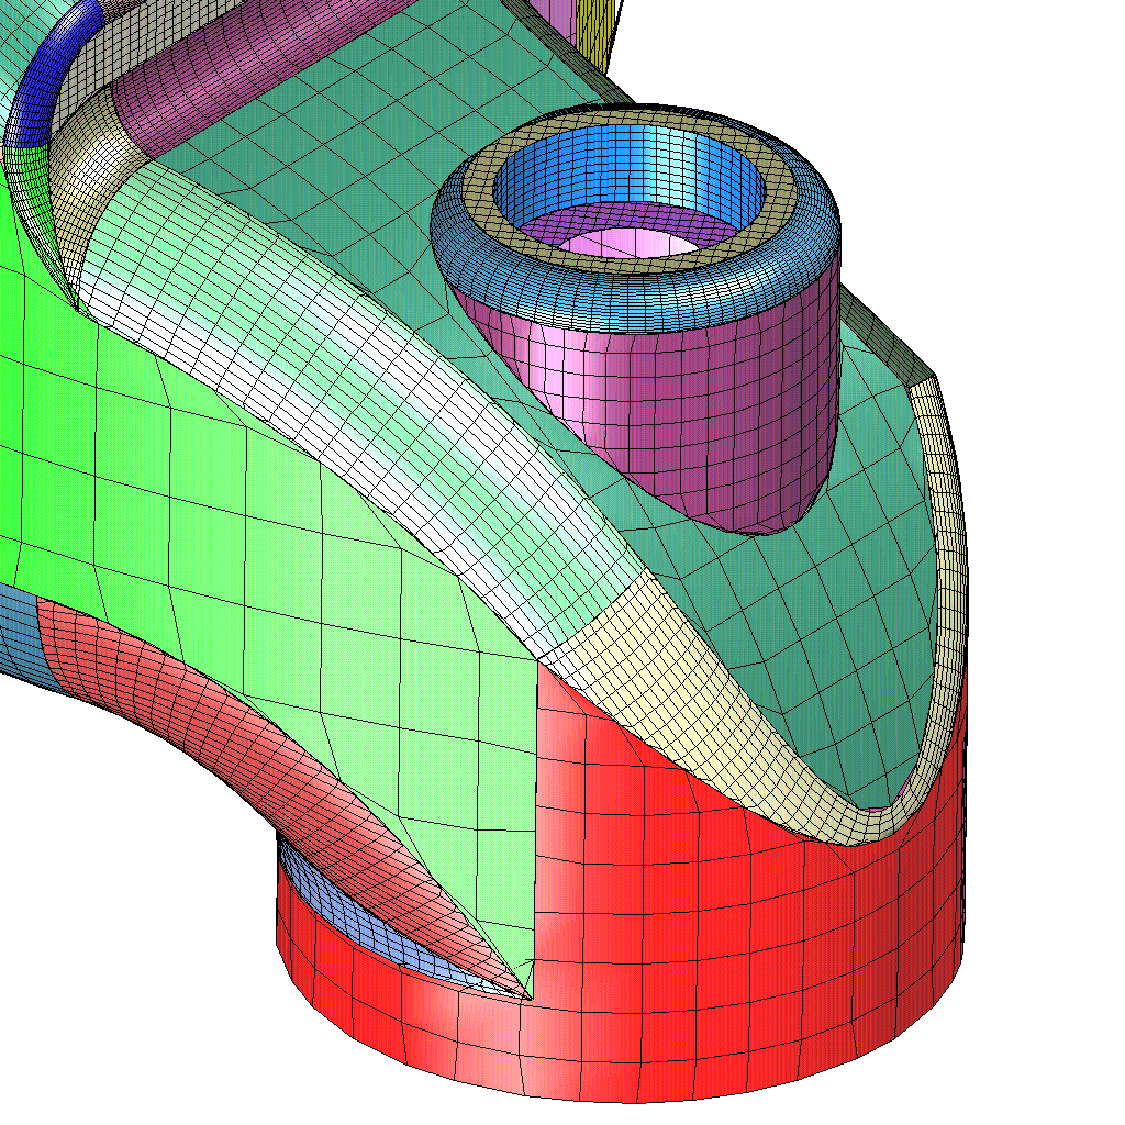
\epsfig{file=\figures/valveExit-cs.ps,height=.5\linewidth}  \\
%- 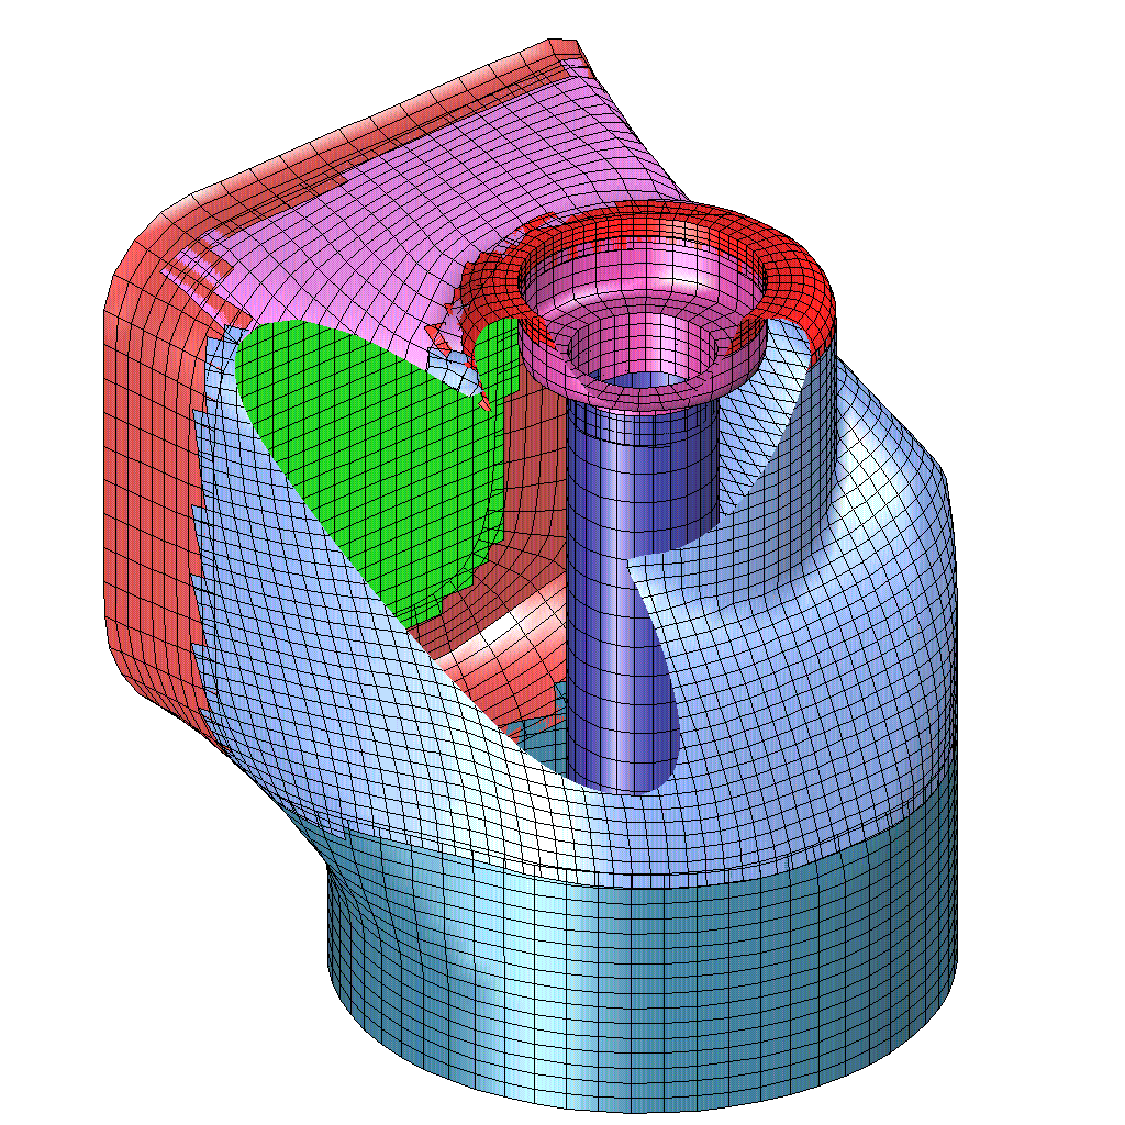
\epsfig{file=\figures/valveExit.ps,height=.5\linewidth}  \\
%- {An overlapping grid (bottom) generated on a portion of the CAD surface (top). Most of the component grids
%- that make up the overlapping grid were generated with the hyperbolic grid generator.}
%- \end{center}




\clearpage
% -------------------------------------------------------------------------------------------------------------------------
\subsection{Bump}

% \renewcommand{\figures}{/home/henshaw/res/mapping}

These figures show a hyperbolic grid generated in both directions
from a smooth spline. The effect of changing various parameters
is demonstrated. See the command file {\tt Overture/sampleMappings/hypeBump.cmd}

{
\newcommand{\figWidthd}{8cm}
\newcommand{\trimfig}[2]{\trimPlotb{#1}{#2}{.0}{.0}{.2}{.0}}
\begin{figure}[hbt]
\begin{center}
\begin{tikzpicture}[scale=1]
  \useasboundingbox (0,.5) rectangle (16.,19.5); % set the bounding box (so we have less surrounding white space)
%
  \draw ( 0.0,0.) node[anchor=south west,xshift=-4pt,yshift=+0pt] {\trimfig{\figures/hypeBump5}{\figWidthd}};
  \draw ( 8.0,0.) node[anchor=south west,xshift=-4pt,yshift=+0pt] {\trimfig{\figures/hypeBump6}{\figWidthd}};
%
  \draw ( 0.0,6.5) node[anchor=south west,xshift=-4pt,yshift=+0pt] {\trimfig{\figures/hypeBump3}{\figWidthd}};
  \draw ( 8.0,6.5) node[anchor=south west,xshift=-4pt,yshift=+0pt] {\trimfig{\figures/hypeBump4}{\figWidthd}};
%
  \draw ( 0.0,13.) node[anchor=south west,xshift=-4pt,yshift=+0pt] {\trimfig{\figures/hypeBump1}{\figWidthd}};
  \draw ( 8.0,13.) node[anchor=south west,xshift=-4pt,yshift=+0pt] {\trimfig{\figures/hypeBump2}{\figWidthd}};
%
 % \draw (current bounding box.south west) rectangle (current bounding box.north east);
% grid:
% \draw[step=1cm,gray] (0,0) grid (16,19);
\end{tikzpicture}
\end{center}
\caption{Hyperbolic grids generated using different values of the papers (noted in the titles)}
\end{figure}
}



\clearpage
% ---------------------------------------------------------------------------------------------------------------
\subsection{Flat Plate}

A spline is built to define a 'flat plate' with rounded edges.
The shape preserving option is used with the spline which allows
only a few knots to define the spline. A hypebolic grid is grown
starting from the spline. The figures show the resulting grids
as various parameters are changed.
See the command file {\tt Overture/sampleMappings/hypeLine.cmd}

{
\newcommand{\figWidthd}{7.5cm}
\newcommand{\trimfig}[2]{\trimPlotb{#1}{#2}{.0}{.0}{.15}{.0}}
\begin{figure}[hbt]
\begin{center}
\begin{tikzpicture}[scale=1]
  \useasboundingbox (0,.5) rectangle (16.,19.5); % set the bounding box (so we have less surrounding white space)
%
  \draw ( 0.0,0.) node[anchor=south west,xshift=-4pt,yshift=+0pt] {\trimfig{\figures/hypeLine5}{\figWidthd}};
  \draw ( 8.0,0.) node[anchor=south west,xshift=-4pt,yshift=+0pt] {\trimfig{\figures/hypeLine6}{\figWidthd}};
%
  \draw ( 0.0,6.5) node[anchor=south west,xshift=-4pt,yshift=+0pt] {\trimfig{\figures/hypeLine3}{\figWidthd}};
  \draw ( 8.0,6.5) node[anchor=south west,xshift=-4pt,yshift=+0pt] {\trimfig{\figures/hypeLine4}{\figWidthd}};
%
  \draw ( 0.0,13.) node[anchor=south west,xshift=-4pt,yshift=+0pt] {\trimfig{\figures/hypeLine1}{\figWidthd}};
  \draw ( 8.0,13.) node[anchor=south west,xshift=-4pt,yshift=+0pt] {\trimfig{\figures/hypeLine2}{\figWidthd}};
%
 % \draw (current bounding box.south west) rectangle (current bounding box.north east);
% grid:
% \draw[step=1cm,gray] (0,0) grid (16,19);
\end{tikzpicture}
\end{center}
\caption{Hyperbolic grids generated using different values of the papers (noted in the titles)}
\end{figure}
}




\clearpage
% ---------------------------------------------------------------------------------------------------------------
\subsection{Mast for a sail}
This example shows the use of the `match to a mapping' boundary condition.
In this case the boundary condition for the hyperbolic marching is that the 
boundary points should lie on some other specified Mapping.
See the command file {\tt Overture/sampleMappings/mastSail2d.cmd}

{
\newcommand{\figWidthd}{7.5cm}
\newcommand{\trimfig}[2]{\trimPlot{#1}{#2}{.0}{.0}{.025}{.025}}
\begin{figure}[hbt]
\begin{center}
\begin{tikzpicture}[scale=1]
  \useasboundingbox (0,.5) rectangle (16.,15.0); % set the bounding box (so we have less surrounding white space)
%
  \draw ( 0.0,7.5) node[anchor=south west,xshift=-4pt,yshift=+0pt] {\trimfig{\figures/mastSail2d_mast}{\figWidthd}};
  \draw (4.0,7.5) node[draw,fill=white,anchor=south,yshift=+0pt] {\small Mapping defining a mast};
  \draw (8.0,7.5) node[anchor=south west,xshift=-4pt,yshift=+0pt] {\trimfig{\figures/mastSail2d_mastGrid}{\figWidthd}};
  \draw (12.0,7.5) node[draw,fill=white,anchor=south,yshift=+0pt] {\parbox{6cm}{\small A hyperbolic grid is marched starting from the mast and matching to the sail}};
%
  \draw ( 0.0,0.) node[anchor=south west,xshift=-4pt,yshift=+0pt] {\trimfig{\figures/mastSail2d_mastAndSail}{\figWidthd}};
  \draw (4.0,0.5) node[draw,fill=white,anchor=south,yshift=+0pt] {\parbox{6cm}{\small Hyperbolic grids created for a mast attached to a sail}};
%
 % \draw (current bounding box.south west) rectangle (current bounding box.north east);
% grid:
% \draw[step=1cm,gray] (0,0) grid (16,15);
\end{tikzpicture}
\end{center}
\caption{Hyperbolic grids generated for a mast and sail.}
\end{figure}
}



\clearpage
% ---------------------------------------------------------------------------------------------------------------
\subsection{Airfoil grids}

The {\tt AirfoilMapping} can be used to generate various types of airfoil shapes. 
These shapes can be used as starting curves for the hypebolic grid generator.
Some care must be taken at the trailing edge since the curvature is so large.
The boundary condition `{\tt trailing edge}' is specified so the grid generator
can choose a good marching direction at the trailing edge. 

See the command file {\tt Overture/sampleMappings/hypeNaca.cmd}


{
\newcommand{\figWidthd}{7.5cm}
\newcommand{\trimfig}[2]{\trimPlotb{#1}{#2}{.0}{.0}{.025}{.025}}
\begin{figure}[hbt]
\begin{center}
\begin{tikzpicture}[scale=1]
  \useasboundingbox (0,.5) rectangle (16.,15.0); % set the bounding box (so we have less surrounding white space)
%
  \draw ( 0.0,7.5) node[anchor=south west,xshift=-4pt,yshift=+0pt] {\trimfig{\figures/hypeNaca0012}{\figWidthd}};
  \draw (4.0,7.5) node[draw,fill=white,anchor=south,yshift=+0pt] {\small NACA0012, geometric stretching.};
  \draw (8.0,7.5) node[anchor=south west,xshift=-4pt,yshift=+0pt] {\trimfig{\figures/hypeNaca0012_te}{\figWidthd}};
  \draw (12.0,7.5) node[draw,fill=white,anchor=south,yshift=+0pt] {\parbox{6cm}{\small NACA0012, geometric stretching, blowup of the trailing edge.}};
%
  \draw ( 0.0,0.) node[anchor=south west,xshift=-4pt,yshift=+0pt] {\trimfig{\figures/hypeNaca1012}{\figWidthd}};
  \draw (4.0,0.5) node[draw,fill=white,anchor=south,yshift=+0pt] {\parbox{6cm}{\small NACA1012, geometric stretching}};
%
  \draw ( 8.0,0.) node[anchor=south west,xshift=-4pt,yshift=+0pt] {\trimfig{\figures/hypeNaca1012_te}{\figWidthd}};
  \draw (12.,0.5) node[draw,fill=white,anchor=south,yshift=+0pt] {\parbox{6cm}{\small NACA1012, geometric stretching, blowup of the trailing edge.}};
%
%\draw (current bounding box.south west) rectangle (current bounding box.north east);
% grid:
% \draw[step=1cm,gray] (0,0) grid (16,15);
\end{tikzpicture}
\end{center}
\caption{Hyperbolic grids generated for NACA airfoils.}
\end{figure}
}




\clearpage
% ---------------------------------------------------------------------------------------------------------------
\subsection{Surface grid generation on a CompositeSurface for a soup can}

In this example we first build a CompositeSurface for a soup can consisting of two subsurfaces.
A surface grid is then generated around the edge. A volume grid is grown outward from the
surface grid.
See the command file {\tt Overture/sampleMappings/hypeCan.cmd}


{
\newcommand{\figWidthd}{7.5cm}
\newcommand{\trimfig}[2]{\trimPlot{#1}{#2}{.0}{.0}{.0}{.025}}
\begin{figure}[hbt]
\begin{center}
\begin{tikzpicture}[scale=1]
  \useasboundingbox (0,.5) rectangle (16.,15.0); % set the bounding box (so we have less surrounding white space)
%
  \draw ( 0.0,7.5) node[anchor=south west,xshift=-4pt,yshift=+0pt] {\trimfig{\figures/hypeCan_rf}{\figWidthd}};
  \draw (4.0,7.5) node[draw,fill=white,anchor=south,yshift=+0pt] {\small Reference surface is a CompositeSurface};
  \draw (8.0,7.5) node[anchor=south west,xshift=-4pt,yshift=+0pt] {\trimfig{\figures/hypeCan_surf}{\figWidthd}};
  \draw (12.0,7.5) node[draw,fill=white,anchor=south,yshift=+0pt] {\parbox{6cm}{\small Surface grid grown in both directions from the corner.}};
%
  \draw ( 0.0,0.) node[anchor=south west,xshift=-4pt,yshift=+0pt] {\trimfig{\figures/hypeCan_vol}{\figWidthd}};
  \draw (4.0,0.5) node[draw,fill=white,anchor=south,yshift=+0pt] {\parbox{6cm}{\small Volume grid grown outward from the surface grid.}};
%
 % \draw (current bounding box.south west) rectangle (current bounding box.north east);
% grid:
% \draw[step=1cm,gray] (0,0) grid (16,15);
\end{tikzpicture}
\end{center}
\caption{Hyperbolic grids generated for a {\em soup can}.}
\end{figure}
}



\clearpage
% ---------------------------------------------------------------------------------------------------------------
\subsection{Surface and Volume Grid Generation on a CAD model for an Automobile.}

Figure~(\ref{fig:asmo}) show an overlapping grid for the {\it ASMO} prototype
automobile. The geometry of the asmo is defined by a CAD model and saved
in an IGES file. 

Creating an overlapping grid for this geometry requires some experience in using the
various tools - {\bf rap} for CAD fixup, {\bf mbuilder} for building mappings and hyperbolic grids
and {\bf ogen}, the overlapping grid generator.

Here are the steps taken to build the grid for the asmo. The steps will use the
command files {\tt asmoNoWheels.cmd}, {\tt asmoBody.cmd}, {\tt asmoFrontWheel.cmd},
{\tt asmoBackWheel.cmd} and {\tt asmo.cmd} found in the {\tt Overture/sampleGrids}
directory. They will also use the {\bf rap}, {\bf mbuilder} and {\bf ogen} programs found
in the {\tt Overture/bin} directory. The IGES file defining the asmo CAD geometry is found in 
{\tt Overture/\-sample\-Mappings/\-asmo.igs}.

\noindent{\bf Step 1. CAD cleanup with rap}: The {\bf rap} program is used to build a version
of the asmo without any wheels by running ``rap asmoNoWheels.cmd''. This program will pause
at various stages so you can see what it does. It will create the file {\tt asmoNoWheels.hdf}.
The CAD model has duplicate surfaces which are deleted. After deleting the wheels the holes
in the body are filled in by deleting trimming curves. After cleanup the 
connectivity is determined and a global triangulation is built.
Refer to publications\cite{cadProjection01,Petersson01} for further details of the CAD fixup and
connectivity algorithms. These are available from the Overture web page, under publications.
 

\noindent{\bf Step 2. Grids for the body}: Running ``mbuilder asmoBody.cmd'' will generate grids
around the body of the asmo. The file {\tt asmoNoWheels.hdf} built in step 1. will be read in. 
The file {\tt asmoBody.hdf} will be created. The {\tt mbuilder} program
will use the {\bf MappingBuilder} class to coordinate the construction of grids on 
the CAD surface. Body fitted grids are built by choosing a starting curve on the surface,
growing a surface grid from this start curve and then generating a volume grid from the
surface grid. The aim was to build a few number of high quality grids.
We also build a large cartesian box to place the car in.

\noindent{\bf Step 3. Grids for the wheels}: Running ``mbuilder asmoFrontWheel.cmd'' and
``mbuilder asmoBackWheel.cmd'' will generate grids for the front wheel and back wheel and
create the files {\tt asmoFrontWheel.hdf} and {\tt asmoBackWheel.hdf}.
These command files will directly read the asmo IGES file {\tt asmo.igs} and select a subset
of the surfaces to work on since it is faster to work with a smaller geometry.
The trimmed surfaces near the rear wheel do not match very well
and the surface has to be repaired.

\noindent{\bf Step 4. Overlapping grid}: Running ``ogen asmo.cmd'' will build the
overlapping grid for the asmo. It will read the component grids generated by the previous steps.
When the asmo grid was made for the first time, the wheels were left off in order to
simplify the grid generation. The wheels were then added, one at a time. This is in general a good
approach to use: slowly build up the grid for a complicated geometry starting from a simplified version.

% \begin{description}
%   \item[CAD fixup] : The CAD model was read in and the geometry was fixed, file {\tt asmo.cmd}.
%                      The CAD model had duplicate surfaces which were deleted and the trimmed
%                      surfaces around the rear wheel did not match very well.
%                      The connectivity was determined and a global triangulation was built.
%                      Refer to publication\cite{imr10} for further details of th CAD fixup and
%                      connectivity algorithms. The corrected model is saved in a data-base file.
%   \item[Surface and Volume Grid Generation]: The surface and volume
%         grid generation was split into 3 steps. In the first
%     step the wheels were ignored and grids were built for the body, front an rear. 
%     The aim was to build a few number of high quality grids. The command file {\tt asmoBody.cmd}
%     builds grids for the body. In the second and third steps grids where made for the front
%     and back wheels using the command files {\tt asmoFrontWheel.cmd} and {\tt asmoRearWheel.cmd}.
%     We also build a large cartesian box to place the car in.
%   \item[Overlapping grid generation] : The command file {\tt asmo.cmd} is used to build the 
%      overlapping grid. When this grid was first made the wheels were left off in order to
%      simplify the grid generation. The wheels were then added, one at a time. 
% \end{description}


{
\newcommand{\figWidthd}{7.5cm}
\newcommand{\trimfig}[2]{\trimPlotb{#1}{#2}{.0}{.0}{.0}{.0}}
\begin{figure}[hbt]
\begin{center}
\begin{tikzpicture}[scale=1]
  \useasboundingbox (0,.5) rectangle (16.,15.0); % set the bounding box (so we have less surrounding white space)
%
  \draw ( 0.0,7.5) node[anchor=south west,xshift=-4pt,yshift=+0pt] {\trimfig{\figures/asmoSurface}{\figWidthd}};
  \draw (4.0,7.5) node[draw,fill=white,anchor=south,yshift=+3pt] {\parbox{6cm}{\small CAD geometry for a car consisting of a patched surface.}};
  \draw (8.0,7.5) node[anchor=south west,xshift=-4pt,yshift=+0pt] {\trimfig{\figures/asmoSurfaceTriangulation}{\figWidthd}};
  \draw (12.0,7.5) node[draw,fill=white,anchor=south,yshift=+3pt] {\parbox{6cm}{\small After the CAD representation is repaired a global triangulation is built.}};
%
  \draw ( 0.0,0.) node[anchor=south west,xshift=-4pt,yshift=+0pt] {\trimfig{\figures/asmoFront}{\figWidthd}};
  \draw (4.0,0.5) node[draw,fill=white,anchor=south,yshift=+0pt] {\parbox{6cm}{\small Overlapping grid for the front.}};
%
  \draw ( 8.0,0.) node[anchor=south west,xshift=-4pt,yshift=+0pt] {\trimfig{\figures/asmoWheels}{\figWidthd}};
  \draw (12.,0.5) node[draw,fill=white,anchor=south,yshift=+0pt] {\parbox{6cm}{\small Overlapping grid for the geometry.}};
%
%\draw (current bounding box.south west) rectangle (current bounding box.north east);
% grid:
% \draw[step=1cm,gray] (0,0) grid (16,15);
\end{tikzpicture}
\end{center}
\caption{Generating a grid on a CAD model for the ASMO car.}
\end{figure}
}

% --------------------------------------------------------------------------
%  ********************** Truck Example **********************************
\clearpage
\input truck.tex

% \clearpage
% \section{Class member functions}
% \input HyperbolicMappingInclude.tex



